\ylDisplay{Magnetpeegel} % Ülesande nimi
{Kristian Kuppart} % Autor
{lahtine} % Voor
{2013} % Aasta
{G 2} % Ülesande nr.
{3} % Raskustase
{
% Teema: Magnetism
\ifStatement
Positiivse laenguga $q$ ja kiirusega $v$ osake liigub ristkülikukujulise riba poole nii, et tema kiirusvektor
moodustab riba normaaliga nurga $\alpha$. Riba paksus on $d$ ja seal paikneb
homogeenne $z$-telje suunaline
magnetväli induktsiooniga $B$ (paberi tasandist meie poole suunatud). Millise maksimaalse
langemisnurga $\alpha_{\mathrm{max}}$ korral
osake veel läbib magnetvälja? On teada, et ribaga risti sellesse sisenev osake
läbiks riba.

\begin{center}
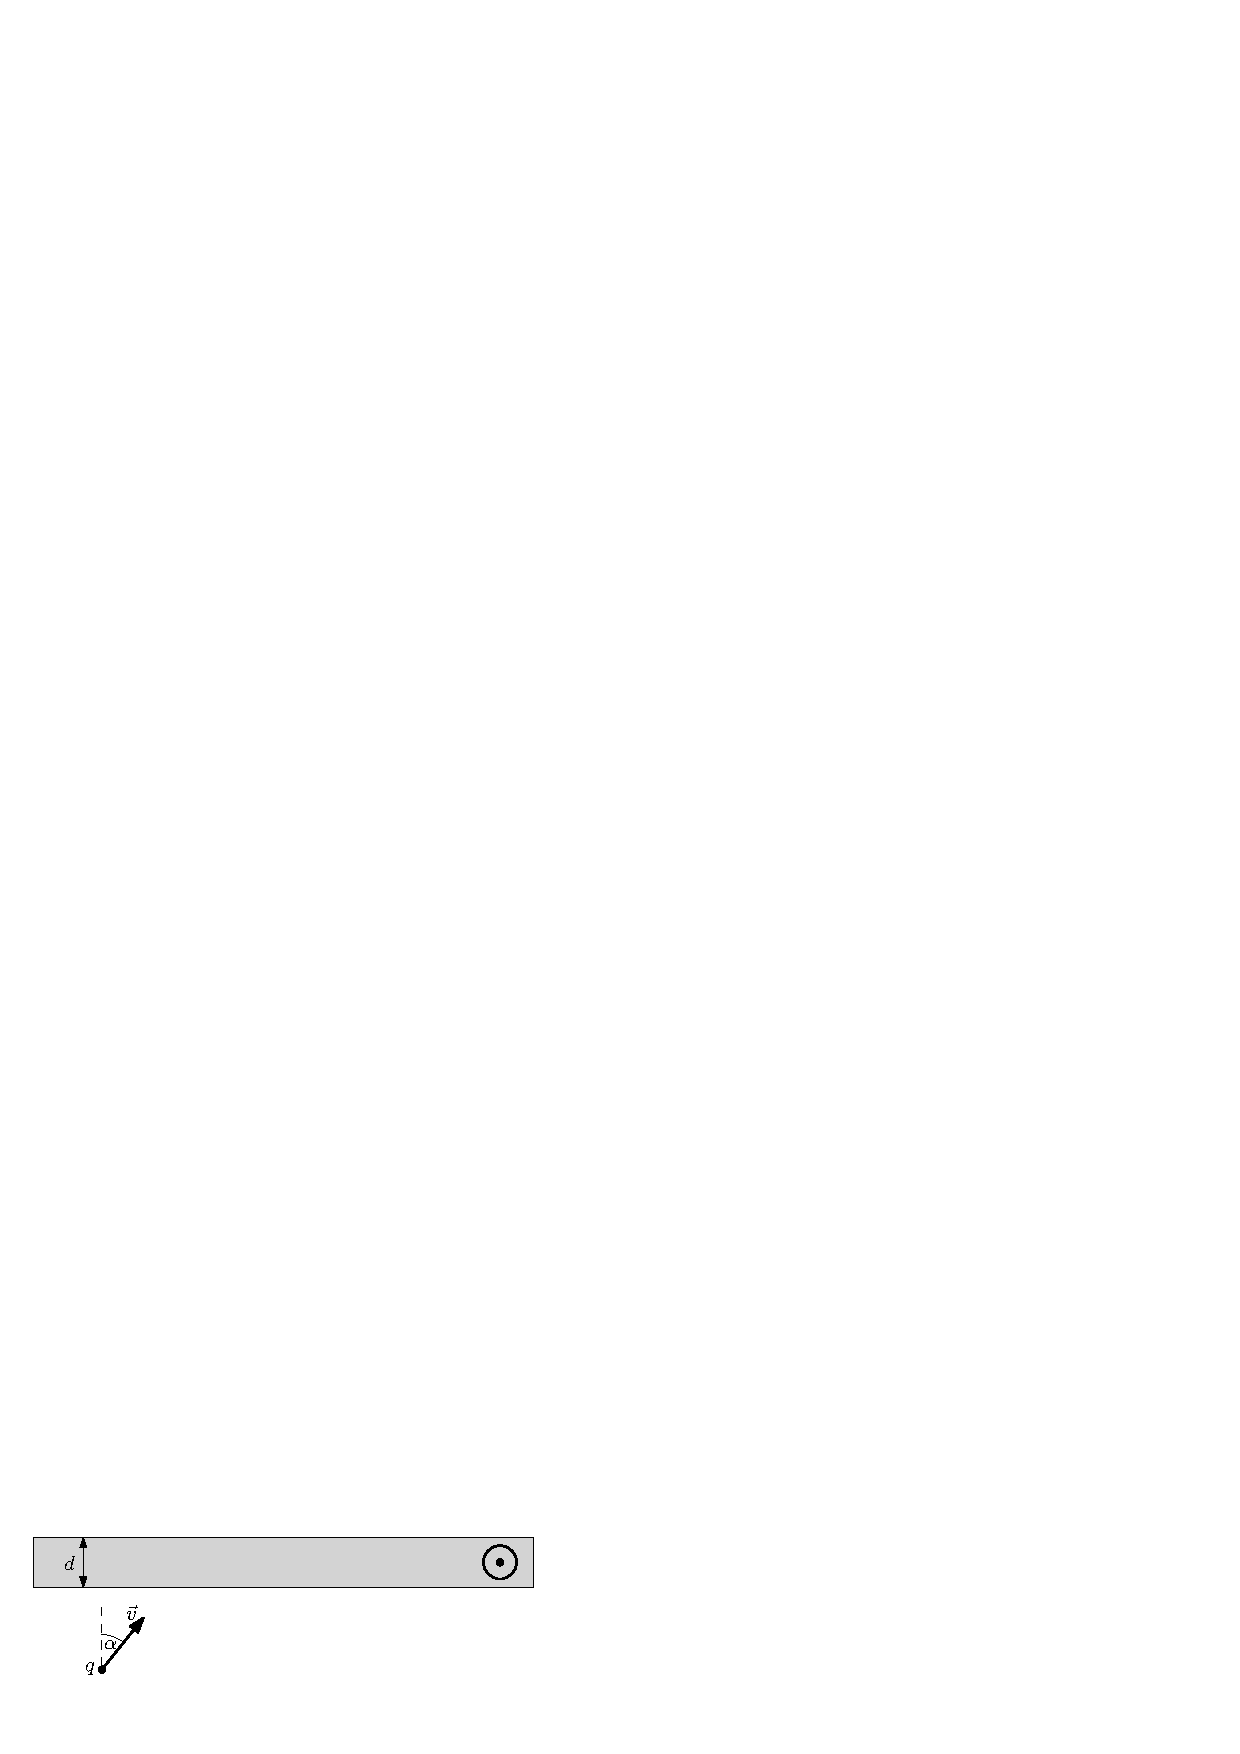
\includegraphics[width=\linewidth]{2013-lahg-02-magnetpeegeljoonis_ipe}
\end{center}
\fi


\ifHint
Magnetväljas hakkab osake liikuma mööda ringjoont, mille raadius on leitav jõudude tasakaalust. Maksimaalse nurga korral väljub osake magnetribast eraldusjoonega paralleelselt.
\fi


\ifSolution
Magenetvälja sattununa hakkab osake liikuma mööda ringjoone kaart, mille kõverusraadiuse saame leida, kui mõtleme, et ringliikumiseks vajaliku kesktõmbejõu annab Lorentzi jõud:
\[m\frac{v^2}{r}=qvB, \quad \text{millest} \quad r=\frac{mv}{qB}.\]
Kui langemisnurk $\alpha$ on piisavalt väike, läbib osake magnetvälja riba. Kui hakkame $\alpha$-t
suurendama, saabub olukord, kus ühel hetkel osake enam magnetvälja riba ei läbi, vaid ``peegeldub'' tagasi. Sellel piirjuhul (vt joonist):

\[r\sin\alpha_\text{max}+d=r, \quad \text{millest} \quad \alpha_\text{max}=\sin^{-1}\left(1-\frac{d}{r}\right).\]

\begin{center}
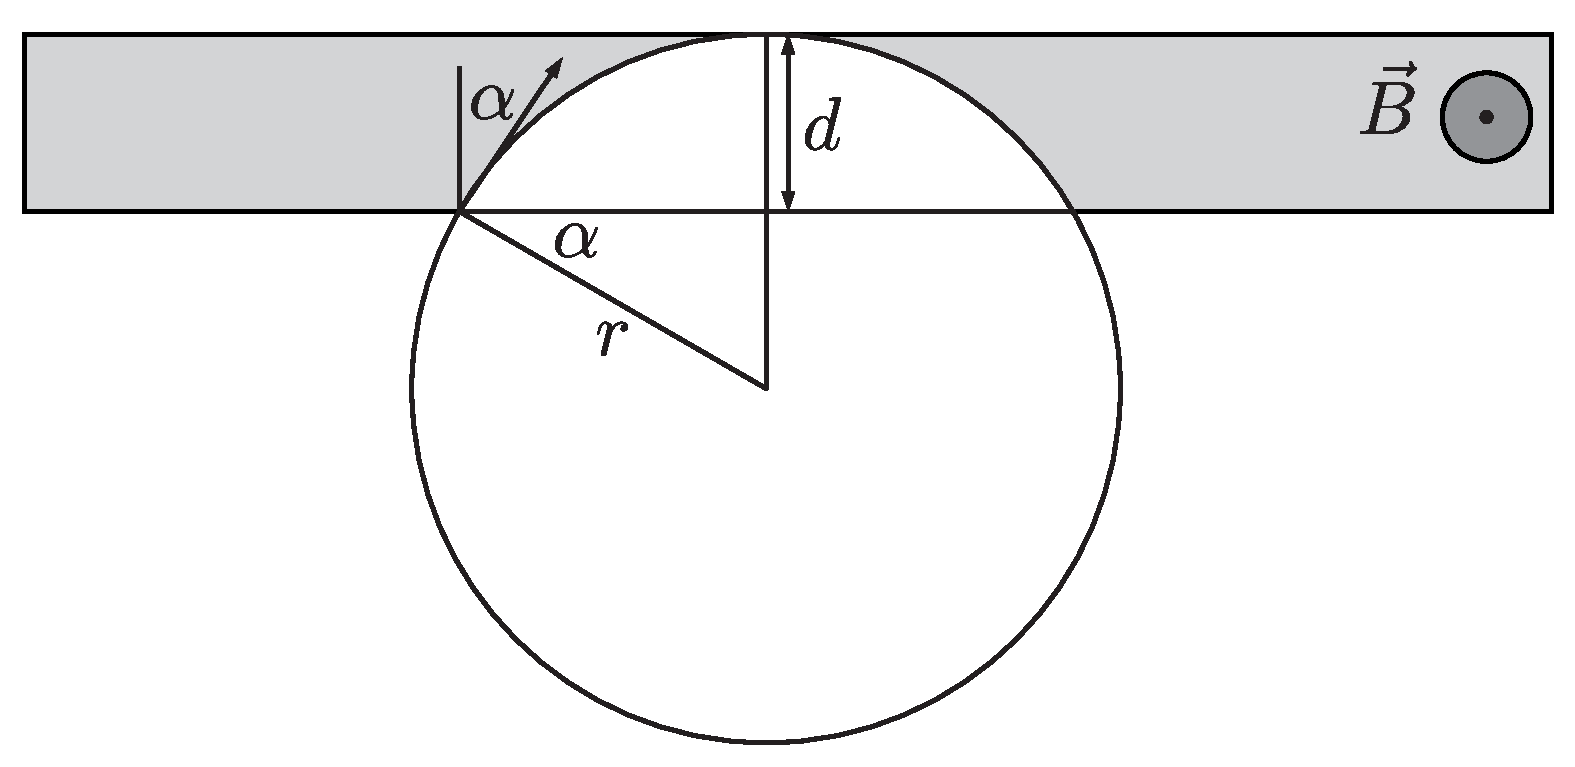
\includegraphics[width=0.9\textwidth]{2013-lahg-02-magPeegLah.pdf}
\end{center}
\fi


\ifEngStatement
% Problem name: Magnet mirror
A particle with a positive charge $q$ and velocity $v$ moves towards a rectangular strip so that that its velocity vector forms an angle $\alpha$ with the normal of the strip. The thickness of the strip is $d$ and on it is located a homogeneous $z$-directional magnetic field with an induction $B$ (from the plane of the paper directed towards us). For what maximal falling angle $\alpha_{\mathrm{max}}$ does the particle still go through the magnetic field? It is known that the particle that enters the strip perpendicularly would go through the strip.
\begin{center}
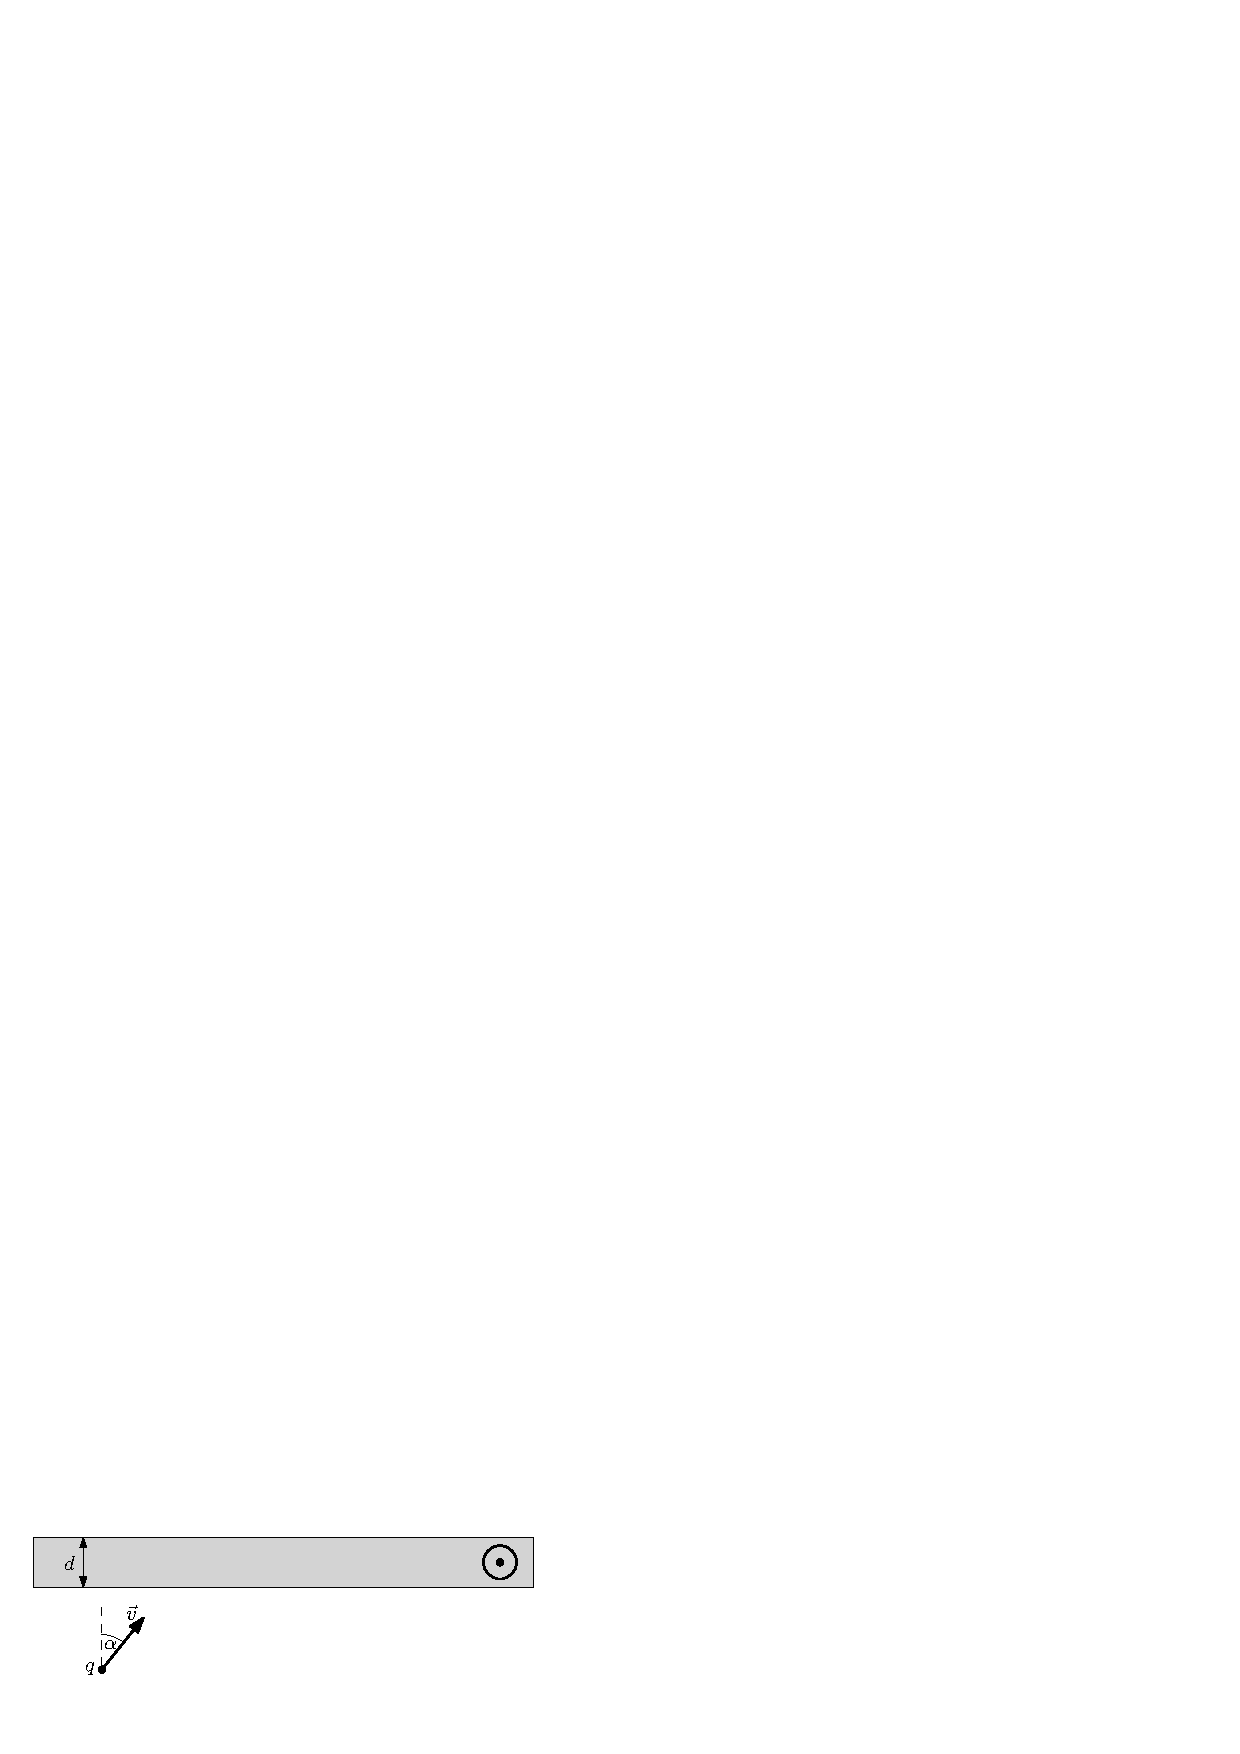
\includegraphics[width=\linewidth]{2013-lahg-02-magnetpeegeljoonis_ipe}
\end{center}
\fi


\ifEngHint
In the magnetic field the particle starts to move along a circle. The radius of the circle can be found from the force balance. If the angle is maximal then the particle leaves the magnetic strip parallel to the separation line.
\fi


\ifEngSolution
After getting into the magnetic field the particle starts to move along a circle. We can find its radius by observing that the centripetal force needed for circular movement is caused by the Lorentz force:
\[m\frac{v^2}{r}=qvB, \quad \text{millest} \quad r=\frac{mv}{qB}.\]
If the falling angle $\alpha$ is small enough the particle goes through the magnetic field strip. If we start to increase $\alpha$ a situation occurs where by one moment the particle does not go through the magnetic field strip but “reflects” back. In this limit case (see figure):
\[r\sin\alpha_\text{max}+d=r, \quad \text{from which} \quad \alpha_\text{max}=\sin^{-1}\left(1-\frac{d}{r}\right).\]
\begin{center}
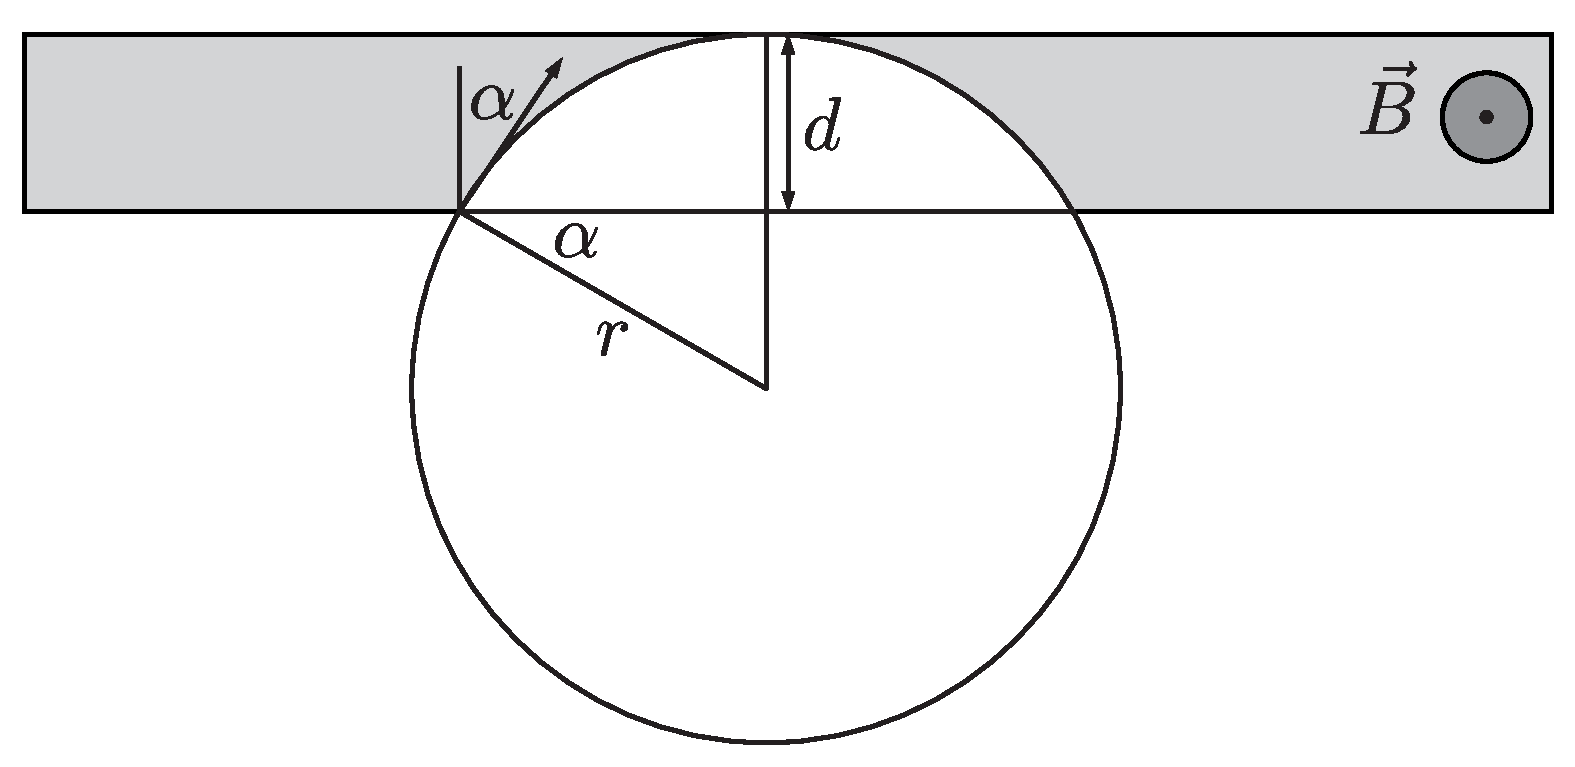
\includegraphics[width=0.9\textwidth]{2013-lahg-02-magPeegLah}
\end{center}
\fi
}